%!TEX root = planning.tex
\section{Function Points: size estimation}
\subsection{Overview} % (fold)
\label{sub:fp_overview}

The \textbf{Function Point approach} is a very useful tool for estimating the effort needed in designing and coding a project. Several aspects are considered for the estimation, as prescribed by the specifications: 
\begin{description}
    \item \textbf{Internal Logic Files}: homogeneous set of data handled by the application being developed;
    \item \textbf{External Interface Files}: homogeneous set of data managed by the application but created elsewhere;
    \item \textbf{External Input}: operation invoked for doing a simple operation on the system with external data (for example, user registration, booking a cab\ldots);
    \item \textbf{External Inquiry}: operation that involves both input and output, mainly for retrieving information from the system;
    \item \textbf{External Output}: system operation producing data for the external environment.
\end{description}

\begin{figure}
\centering
\subfigure[FP Counting Weights]{\label{fig:fp_counting}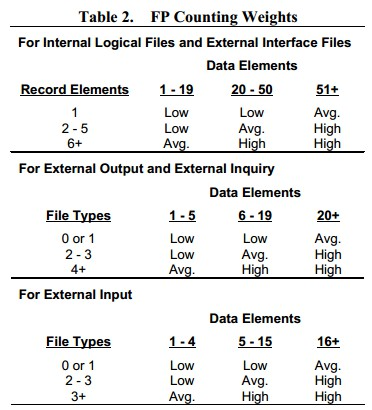
\includegraphics[width=60mm]{img/fpcounting.jpg}}
\subfigure[UFP Complexity Weights]{\label{fig:fp_total}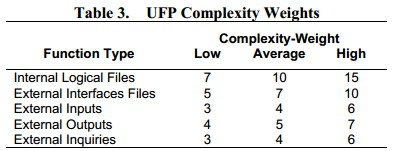
\includegraphics[width=60mm]{img/fptotal.jpg}}
\caption{FP Analysis}
\end{figure}

For each point a \textbf{counting weight} (\emph{Low}, \emph{Avg.} or \emph{High}) has been given according to the parameters specified in Figure~\ref{fig:fp_counting}. After that, a certain amount of FPs has been calculated for each section according to Figure~\ref{fig:fp_total}.

Finally, starting from the total amount of FP, we estimated the project size in KLOC (for more on this, see Section~\ref{sub:results}).

\subsection{Internal Logic Files} % (fold)
\label{sub:ilf}

\subsection{External Interface File} % (fold)
\label{sub:elf}

\subsection{External Input} % (fold)
\label{sub:ei}

\subsection{External Inquiry} % (fold)
\label{sub:eiq}

\subsection{External Output} % (fold)
\label{sub:eo}

\subsection{Results} % (fold)
\label{sub:results}
